\documentclass{article}

% latex packages, feel free to add more here like 'tikz'
\usepackage{style/conference}
\usepackage{opensans}
\usepackage{graphicx}
\graphicspath{{./figures/}}
\usepackage[sorting=none]{biblatex}
\usepackage{fontawesome}
\usepackage[hidelinks]{hyperref}

% to reference, paste the BibTeX obtained from google scholar into references.bib
\addbibresource{references.bib}
%%%%% NEW MATH DEFINITIONS %%%%%

\usepackage{amsmath,amsfonts,bm}

% Mark sections of captions for referring to divisions of figures
\newcommand{\figleft}{{\em (Left)}}
\newcommand{\figcenter}{{\em (Center)}}
\newcommand{\figright}{{\em (Right)}}
\newcommand{\figtop}{{\em (Top)}}
\newcommand{\figbottom}{{\em (Bottom)}}
\newcommand{\captiona}{{\em (a)}}
\newcommand{\captionb}{{\em (b)}}
\newcommand{\captionc}{{\em (c)}}
\newcommand{\captiond}{{\em (d)}}

% Highlight a newly defined term
\newcommand{\newterm}[1]{{\bf #1}}


% Figure reference, lower-case.
\def\figref#1{figure~\ref{#1}}
% Figure reference, capital. For start of sentence
\def\Figref#1{Figure~\ref{#1}}
\def\twofigref#1#2{figures \ref{#1} and \ref{#2}}
\def\quadfigref#1#2#3#4{figures \ref{#1}, \ref{#2}, \ref{#3} and \ref{#4}}
% Section reference, lower-case.
\def\secref#1{section~\ref{#1}}
% Section reference, capital.
\def\Secref#1{Section~\ref{#1}}
% Reference to two sections.
\def\twosecrefs#1#2{sections \ref{#1} and \ref{#2}}
% Reference to three sections.
\def\secrefs#1#2#3{sections \ref{#1}, \ref{#2} and \ref{#3}}
% Reference to an equation, lower-case.
\def\eqref#1{equation~\ref{#1}}
% Reference to an equation, upper case
\def\Eqref#1{Equation~\ref{#1}}
% A raw reference to an equation---avoid using if possible
\def\plaineqref#1{\ref{#1}}
% Reference to a chapter, lower-case.
\def\chapref#1{chapter~\ref{#1}}
% Reference to an equation, upper case.
\def\Chapref#1{Chapter~\ref{#1}}
% Reference to a range of chapters
\def\rangechapref#1#2{chapters\ref{#1}--\ref{#2}}
% Reference to an algorithm, lower-case.
\def\algref#1{algorithm~\ref{#1}}
% Reference to an algorithm, upper case.
\def\Algref#1{Algorithm~\ref{#1}}
\def\twoalgref#1#2{algorithms \ref{#1} and \ref{#2}}
\def\Twoalgref#1#2{Algorithms \ref{#1} and \ref{#2}}
% Reference to a part, lower case
\def\partref#1{part~\ref{#1}}
% Reference to a part, upper case
\def\Partref#1{Part~\ref{#1}}
\def\twopartref#1#2{parts \ref{#1} and \ref{#2}}

\def\ceil#1{\lceil #1 \rceil}
\def\floor#1{\lfloor #1 \rfloor}
\def\1{\bm{1}}
\newcommand{\train}{\mathcal{D}}
\newcommand{\valid}{\mathcal{D_{\mathrm{valid}}}}
\newcommand{\test}{\mathcal{D_{\mathrm{test}}}}

\def\eps{{\epsilon}}


% Random variables
\def\reta{{\textnormal{$\eta$}}}
\def\ra{{\textnormal{a}}}
\def\rb{{\textnormal{b}}}
\def\rc{{\textnormal{c}}}
\def\rd{{\textnormal{d}}}
\def\re{{\textnormal{e}}}
\def\rf{{\textnormal{f}}}
\def\rg{{\textnormal{g}}}
\def\rh{{\textnormal{h}}}
\def\ri{{\textnormal{i}}}
\def\rj{{\textnormal{j}}}
\def\rk{{\textnormal{k}}}
\def\rl{{\textnormal{l}}}
% rm is already a command, just don't name any random variables m
\def\rn{{\textnormal{n}}}
\def\ro{{\textnormal{o}}}
\def\rp{{\textnormal{p}}}
\def\rq{{\textnormal{q}}}
\def\rr{{\textnormal{r}}}
\def\rs{{\textnormal{s}}}
\def\rt{{\textnormal{t}}}
\def\ru{{\textnormal{u}}}
\def\rv{{\textnormal{v}}}
\def\rw{{\textnormal{w}}}
\def\rx{{\textnormal{x}}}
\def\ry{{\textnormal{y}}}
\def\rz{{\textnormal{z}}}

% Random vectors
\def\rvepsilon{{\mathbf{\epsilon}}}
\def\rvtheta{{\mathbf{\theta}}}
\def\rva{{\mathbf{a}}}
\def\rvb{{\mathbf{b}}}
\def\rvc{{\mathbf{c}}}
\def\rvd{{\mathbf{d}}}
\def\rve{{\mathbf{e}}}
\def\rvf{{\mathbf{f}}}
\def\rvg{{\mathbf{g}}}
\def\rvh{{\mathbf{h}}}
\def\rvu{{\mathbf{i}}}
\def\rvj{{\mathbf{j}}}
\def\rvk{{\mathbf{k}}}
\def\rvl{{\mathbf{l}}}
\def\rvm{{\mathbf{m}}}
\def\rvn{{\mathbf{n}}}
\def\rvo{{\mathbf{o}}}
\def\rvp{{\mathbf{p}}}
\def\rvq{{\mathbf{q}}}
\def\rvr{{\mathbf{r}}}
\def\rvs{{\mathbf{s}}}
\def\rvt{{\mathbf{t}}}
\def\rvu{{\mathbf{u}}}
\def\rvv{{\mathbf{v}}}
\def\rvw{{\mathbf{w}}}
\def\rvx{{\mathbf{x}}}
\def\rvy{{\mathbf{y}}}
\def\rvz{{\mathbf{z}}}

% Elements of random vectors
\def\erva{{\textnormal{a}}}
\def\ervb{{\textnormal{b}}}
\def\ervc{{\textnormal{c}}}
\def\ervd{{\textnormal{d}}}
\def\erve{{\textnormal{e}}}
\def\ervf{{\textnormal{f}}}
\def\ervg{{\textnormal{g}}}
\def\ervh{{\textnormal{h}}}
\def\ervi{{\textnormal{i}}}
\def\ervj{{\textnormal{j}}}
\def\ervk{{\textnormal{k}}}
\def\ervl{{\textnormal{l}}}
\def\ervm{{\textnormal{m}}}
\def\ervn{{\textnormal{n}}}
\def\ervo{{\textnormal{o}}}
\def\ervp{{\textnormal{p}}}
\def\ervq{{\textnormal{q}}}
\def\ervr{{\textnormal{r}}}
\def\ervs{{\textnormal{s}}}
\def\ervt{{\textnormal{t}}}
\def\ervu{{\textnormal{u}}}
\def\ervv{{\textnormal{v}}}
\def\ervw{{\textnormal{w}}}
\def\ervx{{\textnormal{x}}}
\def\ervy{{\textnormal{y}}}
\def\ervz{{\textnormal{z}}}

% Random matrices
\def\rmA{{\mathbf{A}}}
\def\rmB{{\mathbf{B}}}
\def\rmC{{\mathbf{C}}}
\def\rmD{{\mathbf{D}}}
\def\rmE{{\mathbf{E}}}
\def\rmF{{\mathbf{F}}}
\def\rmG{{\mathbf{G}}}
\def\rmH{{\mathbf{H}}}
\def\rmI{{\mathbf{I}}}
\def\rmJ{{\mathbf{J}}}
\def\rmK{{\mathbf{K}}}
\def\rmL{{\mathbf{L}}}
\def\rmM{{\mathbf{M}}}
\def\rmN{{\mathbf{N}}}
\def\rmO{{\mathbf{O}}}
\def\rmP{{\mathbf{P}}}
\def\rmQ{{\mathbf{Q}}}
\def\rmR{{\mathbf{R}}}
\def\rmS{{\mathbf{S}}}
\def\rmT{{\mathbf{T}}}
\def\rmU{{\mathbf{U}}}
\def\rmV{{\mathbf{V}}}
\def\rmW{{\mathbf{W}}}
\def\rmX{{\mathbf{X}}}
\def\rmY{{\mathbf{Y}}}
\def\rmZ{{\mathbf{Z}}}

% Elements of random matrices
\def\ermA{{\textnormal{A}}}
\def\ermB{{\textnormal{B}}}
\def\ermC{{\textnormal{C}}}
\def\ermD{{\textnormal{D}}}
\def\ermE{{\textnormal{E}}}
\def\ermF{{\textnormal{F}}}
\def\ermG{{\textnormal{G}}}
\def\ermH{{\textnormal{H}}}
\def\ermI{{\textnormal{I}}}
\def\ermJ{{\textnormal{J}}}
\def\ermK{{\textnormal{K}}}
\def\ermL{{\textnormal{L}}}
\def\ermM{{\textnormal{M}}}
\def\ermN{{\textnormal{N}}}
\def\ermO{{\textnormal{O}}}
\def\ermP{{\textnormal{P}}}
\def\ermQ{{\textnormal{Q}}}
\def\ermR{{\textnormal{R}}}
\def\ermS{{\textnormal{S}}}
\def\ermT{{\textnormal{T}}}
\def\ermU{{\textnormal{U}}}
\def\ermV{{\textnormal{V}}}
\def\ermW{{\textnormal{W}}}
\def\ermX{{\textnormal{X}}}
\def\ermY{{\textnormal{Y}}}
\def\ermZ{{\textnormal{Z}}}

% Vectors
\def\vzero{{\bm{0}}}
\def\vone{{\bm{1}}}
\def\vmu{{\bm{\mu}}}
\def\vtheta{{\bm{\theta}}}
\def\va{{\bm{a}}}
\def\vb{{\bm{b}}}
\def\vc{{\bm{c}}}
\def\vd{{\bm{d}}}
\def\ve{{\bm{e}}}
\def\vf{{\bm{f}}}
\def\vg{{\bm{g}}}
\def\vh{{\bm{h}}}
\def\vi{{\bm{i}}}
\def\vj{{\bm{j}}}
\def\vk{{\bm{k}}}
\def\vl{{\bm{l}}}
\def\vm{{\bm{m}}}
\def\vn{{\bm{n}}}
\def\vo{{\bm{o}}}
\def\vp{{\bm{p}}}
\def\vq{{\bm{q}}}
\def\vr{{\bm{r}}}
\def\vs{{\bm{s}}}
\def\vt{{\bm{t}}}
\def\vu{{\bm{u}}}
\def\vv{{\bm{v}}}
\def\vw{{\bm{w}}}
\def\vx{{\bm{x}}}
\def\vy{{\bm{y}}}
\def\vz{{\bm{z}}}

% Elements of vectors
\def\evalpha{{\alpha}}
\def\evbeta{{\beta}}
\def\evepsilon{{\epsilon}}
\def\evlambda{{\lambda}}
\def\evomega{{\omega}}
\def\evmu{{\mu}}
\def\evpsi{{\psi}}
\def\evsigma{{\sigma}}
\def\evtheta{{\theta}}
\def\eva{{a}}
\def\evb{{b}}
\def\evc{{c}}
\def\evd{{d}}
\def\eve{{e}}
\def\evf{{f}}
\def\evg{{g}}
\def\evh{{h}}
\def\evi{{i}}
\def\evj{{j}}
\def\evk{{k}}
\def\evl{{l}}
\def\evm{{m}}
\def\evn{{n}}
\def\evo{{o}}
\def\evp{{p}}
\def\evq{{q}}
\def\evr{{r}}
\def\evs{{s}}
\def\evt{{t}}
\def\evu{{u}}
\def\evv{{v}}
\def\evw{{w}}
\def\evx{{x}}
\def\evy{{y}}
\def\evz{{z}}

% Matrix
\def\mA{{\bm{A}}}
\def\mB{{\bm{B}}}
\def\mC{{\bm{C}}}
\def\mD{{\bm{D}}}
\def\mE{{\bm{E}}}
\def\mF{{\bm{F}}}
\def\mG{{\bm{G}}}
\def\mH{{\bm{H}}}
\def\mI{{\bm{I}}}
\def\mJ{{\bm{J}}}
\def\mK{{\bm{K}}}
\def\mL{{\bm{L}}}
\def\mM{{\bm{M}}}
\def\mN{{\bm{N}}}
\def\mO{{\bm{O}}}
\def\mP{{\bm{P}}}
\def\mQ{{\bm{Q}}}
\def\mR{{\bm{R}}}
\def\mS{{\bm{S}}}
\def\mT{{\bm{T}}}
\def\mU{{\bm{U}}}
\def\mV{{\bm{V}}}
\def\mW{{\bm{W}}}
\def\mX{{\bm{X}}}
\def\mY{{\bm{Y}}}
\def\mZ{{\bm{Z}}}
\def\mBeta{{\bm{\beta}}}
\def\mPhi{{\bm{\Phi}}}
\def\mLambda{{\bm{\Lambda}}}
\def\mSigma{{\bm{\Sigma}}}

% Tensor
\DeclareMathAlphabet{\mathsfit}{\encodingdefault}{\sfdefault}{m}{sl}
\SetMathAlphabet{\mathsfit}{bold}{\encodingdefault}{\sfdefault}{bx}{n}
\newcommand{\tens}[1]{\bm{\mathsfit{#1}}}
\def\tA{{\tens{A}}}
\def\tB{{\tens{B}}}
\def\tC{{\tens{C}}}
\def\tD{{\tens{D}}}
\def\tE{{\tens{E}}}
\def\tF{{\tens{F}}}
\def\tG{{\tens{G}}}
\def\tH{{\tens{H}}}
\def\tI{{\tens{I}}}
\def\tJ{{\tens{J}}}
\def\tK{{\tens{K}}}
\def\tL{{\tens{L}}}
\def\tM{{\tens{M}}}
\def\tN{{\tens{N}}}
\def\tO{{\tens{O}}}
\def\tP{{\tens{P}}}
\def\tQ{{\tens{Q}}}
\def\tR{{\tens{R}}}
\def\tS{{\tens{S}}}
\def\tT{{\tens{T}}}
\def\tU{{\tens{U}}}
\def\tV{{\tens{V}}}
\def\tW{{\tens{W}}}
\def\tX{{\tens{X}}}
\def\tY{{\tens{Y}}}
\def\tZ{{\tens{Z}}}


% Graph
\def\gA{{\mathcal{A}}}
\def\gB{{\mathcal{B}}}
\def\gC{{\mathcal{C}}}
\def\gD{{\mathcal{D}}}
\def\gE{{\mathcal{E}}}
\def\gF{{\mathcal{F}}}
\def\gG{{\mathcal{G}}}
\def\gH{{\mathcal{H}}}
\def\gI{{\mathcal{I}}}
\def\gJ{{\mathcal{J}}}
\def\gK{{\mathcal{K}}}
\def\gL{{\mathcal{L}}}
\def\gM{{\mathcal{M}}}
\def\gN{{\mathcal{N}}}
\def\gO{{\mathcal{O}}}
\def\gP{{\mathcal{P}}}
\def\gQ{{\mathcal{Q}}}
\def\gR{{\mathcal{R}}}
\def\gS{{\mathcal{S}}}
\def\gT{{\mathcal{T}}}
\def\gU{{\mathcal{U}}}
\def\gV{{\mathcal{V}}}
\def\gW{{\mathcal{W}}}
\def\gX{{\mathcal{X}}}
\def\gY{{\mathcal{Y}}}
\def\gZ{{\mathcal{Z}}}

% Sets
\def\sA{{\mathbb{A}}}
\def\sB{{\mathbb{B}}}
\def\sC{{\mathbb{C}}}
\def\sD{{\mathbb{D}}}
% Don't use a set called E, because this would be the same as our symbol
% for expectation.
\def\sF{{\mathbb{F}}}
\def\sG{{\mathbb{G}}}
\def\sH{{\mathbb{H}}}
\def\sI{{\mathbb{I}}}
\def\sJ{{\mathbb{J}}}
\def\sK{{\mathbb{K}}}
\def\sL{{\mathbb{L}}}
\def\sM{{\mathbb{M}}}
\def\sN{{\mathbb{N}}}
\def\sO{{\mathbb{O}}}
\def\sP{{\mathbb{P}}}
\def\sQ{{\mathbb{Q}}}
\def\sR{{\mathbb{R}}}
\def\sS{{\mathbb{S}}}
\def\sT{{\mathbb{T}}}
\def\sU{{\mathbb{U}}}
\def\sV{{\mathbb{V}}}
\def\sW{{\mathbb{W}}}
\def\sX{{\mathbb{X}}}
\def\sY{{\mathbb{Y}}}
\def\sZ{{\mathbb{Z}}}

% Entries of a matrix
\def\emLambda{{\Lambda}}
\def\emA{{A}}
\def\emB{{B}}
\def\emC{{C}}
\def\emD{{D}}
\def\emE{{E}}
\def\emF{{F}}
\def\emG{{G}}
\def\emH{{H}}
\def\emI{{I}}
\def\emJ{{J}}
\def\emK{{K}}
\def\emL{{L}}
\def\emM{{M}}
\def\emN{{N}}
\def\emO{{O}}
\def\emP{{P}}
\def\emQ{{Q}}
\def\emR{{R}}
\def\emS{{S}}
\def\emT{{T}}
\def\emU{{U}}
\def\emV{{V}}
\def\emW{{W}}
\def\emX{{X}}
\def\emY{{Y}}
\def\emZ{{Z}}
\def\emSigma{{\Sigma}}

% entries of a tensor
% Same font as tensor, without \bm wrapper
\newcommand{\etens}[1]{\mathsfit{#1}}
\def\etLambda{{\etens{\Lambda}}}
\def\etA{{\etens{A}}}
\def\etB{{\etens{B}}}
\def\etC{{\etens{C}}}
\def\etD{{\etens{D}}}
\def\etE{{\etens{E}}}
\def\etF{{\etens{F}}}
\def\etG{{\etens{G}}}
\def\etH{{\etens{H}}}
\def\etI{{\etens{I}}}
\def\etJ{{\etens{J}}}
\def\etK{{\etens{K}}}
\def\etL{{\etens{L}}}
\def\etM{{\etens{M}}}
\def\etN{{\etens{N}}}
\def\etO{{\etens{O}}}
\def\etP{{\etens{P}}}
\def\etQ{{\etens{Q}}}
\def\etR{{\etens{R}}}
\def\etS{{\etens{S}}}
\def\etT{{\etens{T}}}
\def\etU{{\etens{U}}}
\def\etV{{\etens{V}}}
\def\etW{{\etens{W}}}
\def\etX{{\etens{X}}}
\def\etY{{\etens{Y}}}
\def\etZ{{\etens{Z}}}

% The true underlying data generating distribution
\newcommand{\pdata}{p_{\rm{data}}}
% The empirical distribution defined by the training set
\newcommand{\ptrain}{\hat{p}_{\rm{data}}}
\newcommand{\Ptrain}{\hat{P}_{\rm{data}}}
% The model distribution
\newcommand{\pmodel}{p_{\rm{model}}}
\newcommand{\Pmodel}{P_{\rm{model}}}
\newcommand{\ptildemodel}{\tilde{p}_{\rm{model}}}
% Stochastic autoencoder distributions
\newcommand{\pencode}{p_{\rm{encoder}}}
\newcommand{\pdecode}{p_{\rm{decoder}}}
\newcommand{\precons}{p_{\rm{reconstruct}}}

\newcommand{\laplace}{\mathrm{Laplace}} % Laplace distribution

\newcommand{\E}{\mathbb{E}}
\newcommand{\Ls}{\mathcal{L}}
\newcommand{\R}{\mathbb{R}}
\newcommand{\emp}{\tilde{p}}
\newcommand{\lr}{\alpha}
\newcommand{\reg}{\lambda}
\newcommand{\rect}{\mathrm{rectifier}}
\newcommand{\softmax}{\mathrm{softmax}}
\newcommand{\sigmoid}{\sigma}
\newcommand{\softplus}{\zeta}
\newcommand{\KL}{D_{\mathrm{KL}}}
\newcommand{\Var}{\mathrm{Var}}
\newcommand{\standarderror}{\mathrm{SE}}
\newcommand{\Cov}{\mathrm{Cov}}
% Wolfram Mathworld says $L^2$ is for function spaces and $\ell^2$ is for vectors
% But then they seem to use $L^2$ for vectors throughout the site, and so does
% wikipedia.
\newcommand{\normlzero}{L^0}
\newcommand{\normlone}{L^1}
\newcommand{\normltwo}{L^2}
\newcommand{\normlp}{L^p}
\newcommand{\normmax}{L^\infty}

\newcommand{\parents}{Pa} % See usage in notation.tex. Chosen to match Daphne's book.

\DeclareMathOperator*{\argmax}{arg\,max}
\DeclareMathOperator*{\argmin}{arg\,min}

\DeclareMathOperator{\sign}{sign}
\DeclareMathOperator{\Tr}{Tr}
\let\ab\allowbreak


% replace this title with your own
\title{A Variational Autoencoder to Generate Winged Horses}

\begin{document}
\maketitle
\begin{abstract}
    This paper proposes using a convolutional variational autoencoder to generate winged horse (Pegasus) images. To achieve this a variational autoencoder is trained on a images of horses and birds to learn a distribution over the data that permits sampling. The experiments performed suggest that this approach is poor at producing these images and produces blurry images that slightly resemble winged horses.
\end{abstract}
% this is where the sections begin
\section{Methodology}
\subsection{Model}
The model used is a convolutional variation autoencoder (VAE)~\cite{vae} this model was chosen as it is a generative model that produces a structured latent space by feeding in input data, allowing for a better understanding of the latent space when compared with a GAN~\cite{latent}. Variational autoencoders work by learning a distribution over the input data and imposing and additional prior distribution over the latent space $p(\bm{Z})$. This distribution is usually, and in the case of this paper, the standard normal distribution meaning $\bm{Z}\sim\mathcal{N}(\textbf{0}, \bm{\mathit{I}})$. This prior is imposed over the learned distribution in an attempt to force a continuous latent space that can be sampled from, as a normal autoencoder could have gaps in the latent space that produce meaningless results when decoded. In order to impose this prior the architecture of a normal autoencoder is modified as described in~\cite{vae} that is rather than the encoder network encoding to latent space $\bm{Z}$ it learns a distribution of encodings for each input parameterised by a mean vector $\bm{\mu}$ and standard deviation vector $\bm{\sigma}$. On every forward pass through the decoder these are combined in a random manner to generate the encoding of the input thus learning a continuous latent space. The manner in which they are combined according to $\bm{z}=\bm{\mu} +\bm{\sigma}\odot\epsilon$ where $\epsilon\sim\mathcal{N}(\bf{0}, \bm{\mathit{I}})$. This is illustrated below in \autoref{fig:arch}:
\begin{figure}[h]
    \centering
    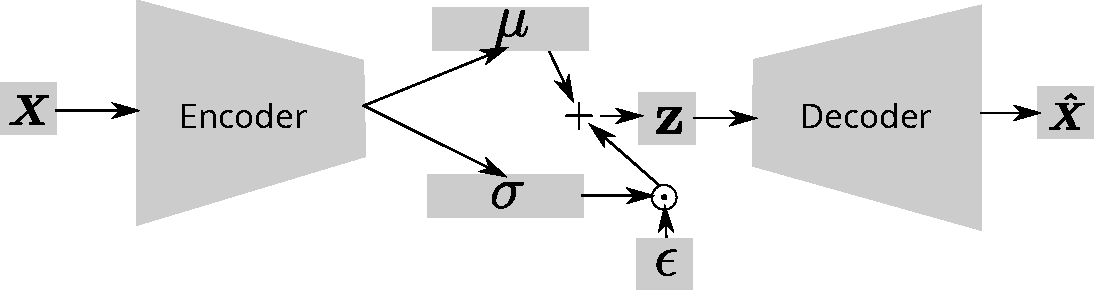
\includegraphics[width=0.6\textwidth]{vae}
    \caption{Diagram of VAE arhcitecture}
    \label{fig:arch}
\end{figure}
\par
The encoder and decoder are both convolutional neural networks (CNN), with 4 convolutional layers and 4 fully connected layers in the encoder and 4 de-convolutional layers and 4 fully connected layers in the decoder. The large number of fully connected layers were used so that after extracting features from the input image using the convolutional layers the network can better learn how these features represent the input images. Qualitative testing showed that random samples from the model had much more realistic colours when compared with the model without the fully connected layers. Between convolutional layers batch normalisation was used as it has been shown to improve convergence time when training as well as act as a normalisation factor~\cite{batch}. The networks activation layers were also chosen to be leaky rectified linear activation units (Leaky ReLU) rather than standard linear rectified activation units (ReLU) as empirical studies have shown that these outperform ReLUs in terms of accuracy~\cite{relu}.
\subsection{Loss Function}
The loss function being minimised for the VAE is as described in~\cite{vae}:
\begin{equation}
    \mathcal{L}_{VAE}=
    -\mathbb{E}_{q(\bm{Z}|\bm{X})}[\log p(\bm{X}|\bm{Z})]
    +D_{KL}(q(\bm{Z}|\bm{X})||p(\bm{Z}))
\end{equation}
where $D_{KL}$ is the Kullback-Leibler divergence and $-\mathbb{E}_{q(\bm{Z}|\bm{X})}$ is the negated expected log-likelihood for each pixel. The negated log-likelihood is equivalent to cross-entropy therefore in the model cross entropy is used in its place. There also exists a closed form solution to $D_{KL}$ as described in~\cite{vae} for the Gaussian distributions such as $\mathcal{N}(\bf{0}, \bm{\mathit{I}})$ being used in the model. It is:
\begin{equation}
    D_{KL}=
    -\frac{1}{2}\sum^{J}_{j=1}
    (1+\log((\sigma_j)^2)-
    (\mu_j)^2-
    (\sigma_j)^2
    )
\end{equation}
The cross-entropy portion of the loss function is a measure of how similar the reconstructed image $\bm{\hat{X}}$ is to the original image $\bm{X}$ whereas the $D_{KL}$ is used to force the resultant encoding distribution to be as close to $\mathcal{N}(\bm{0},\bm{I})$ as possible.
\subsection{Training}
In order to generate the winged horses the model was trained on a mix of the STL-10 dataset~\cite{stl} (resized to 32x32 pixels) and the CIFAR-10 datset~\cite{cifar}. The model was first trained for 100 epochs on the full combined datasets as recommended by~\cite{stl-web} this is done to build a useful prior distribution and learn a diverse set of features for image generation. After this all labelled examples if horses and birds were extracted from the datasets and combined into a new dataset of only horses and birds. The model was then trained on this dataset for 300 more epochs, in order to generate a latent space $\bm{Z}$ that encodes a wide range of features related to horse and bird images, such as wing shape and colour. The optimiser used for the training was the Adam optimiser~\cite{adam} as is standard in the field.
\subsection{Sampling}
There are many approaches to sampling from the latent space $\bm{Z}$, the most naive method would be to randomly sample from the latent space and then decode the samples. If done enough times it is possible that a good image of a winged horse would eventually be produced. However it would be better to take advantage of the structured latent space somehow. Three sampling methods are described in~\cite{sampl}, the most desirable of these would be to take advantage of vector mathematics within the latent space to create an "analogy" vector representing wings within the latent space. This wing vector could then be added to any latent space representation of a horse to generate a winged horse. This was not done as the datasets contained very few images of birds that had wings outstretched clearly and none were labeled as such so this would have required manually picking out all images of birds in flight from a dataset of 115000 images which is highly impractical. Instead interpolation was used to generate the images. Specifically spherical interpolations were used rather than linear interpolations for the reasons stated in~\cite{sampl}, these are that due to the large number of dimensions in the latent space meaning the mid point between 2 points in the space will be many standard deviations from the mean value. Spherical interpolations address this problem by treating the interpolation as a path on a hypersphere~\cite{sampl}. The equation used to perform these interpolations was:
\begin{equation}
    Slerp(q_1,q_2;\bm{\mu})=\frac{\sin[(1-\mu)\theta]}
    {\sin\theta}q_1+
    \frac{\sin\mu\theta}
    {\sin\theta}q_2
\end{equation}
where $\theta=\arccos{q_1\cdot q_2}$ and $q_1, q_2$ are latent vectors.
\par
To generate the batch of 64 winged horse images from the samples a set of 8 horse images were manually selected from the dataset and a set of 21 bird images were also selected. For each horse image a bird image was randomly selected from the bird set and then spherical interpolations were performed with $\mu$ being 8 evenly spaced values from the interval $[0.4, 0.7]$, this interval was chosen as qualitatively it produced results that neither looked completely like the bird or horse image bu instead was clearly a merger of the 2.
\section{Results}
The best batch of winged horses is shown in \autoref{fig:pegs}. The results are quite noisy but nowhere near as much as with a normal autoencoder. The diversity of the batch is not great, however that is to be expected due to the sampling method used to generate the batch, as each row is an interpolation between 2 images so all images in said row will be similar. The vast majority of the images in the sample are white, and the images on rows 4 and 5 do look like winged horses with a small stretch of the imagination.

\begin{figure}[h]
    \centering
    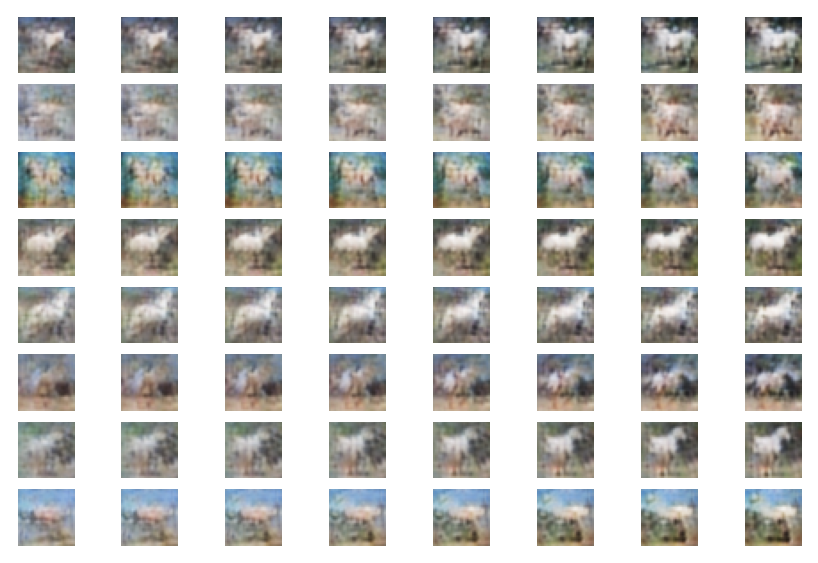
\includegraphics{pegs}
    \caption{Best batch of 64 winged horses from spherical interpolations}
    \label{fig:pegs}
\end{figure}
The best winged horse image from \autoref{fig:pegs} is shown in \autoref{fig:best}
\begin{figure}[h]
    \centering
    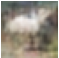
\includegraphics{Best_peg}
    \caption{Best Pegasus image from batch}
    \label{fig:best}
\end{figure}
This depicts a white horse looking at you with its head located in the centre of the image and a clear wing shape in the upper right as well as a less clear wing to the left.
\section{Limitations}
The obvious limitation of the approach presented in this paper is the apparent "blurriness" of the generated images. This blur is actually noise that is caused by using a VAE and manner in which VAEs approximate maximum likelihood~\cite{blur}.
\par
The model also only generates 32x32 pixel images this is due to it only being trained on CIFAR-10 which is already 32x32 and STL-10 which had been resized to 32x32 as a preprocessing step. This was done as training the model on the full resolution (96x96) images from STL-10 took an extremely long amount of time which was not practical due to time constraints.
\par
The chosen sampling method (spherical interpolations) although good was in itself a limitation as better sampling methods for VAEs exist such as Adversarially Constrained Autoencoder Interpolation~\cite{acai}. Unfortunately this method of interpolation is an adversarial method thus would incur the -4 point penalty if used, this may have produced more realistic results but there was no way of knowing if they would be better enough to balance the penalty.
\par
Both CIFAR-10 and STL-10 are very poor datasets with regard to bird images. As a large number of such images are of bird heads or birds that are not in flight (wings not outstretched). This made training the model to represent wings in its latent space very difficult as very few images had those desirable features. For better results a dataset with labeled examples of birds in flight would be far more appropriate.
\section*{Bonuses}
The submission should have a total bonus of +1 as both CIFAR-10 and STL-10 were used albeit at a reduced resolution and nearly all winged horses in the batch (\autoref{fig:pegs}) are white.

% you can have an unlimited number of references (they can go on the 5th page and span many additional pages without any penalty)
\printbibliography
\end{document}